\documentclass[12pt]{article}
\usepackage[utf8]{inputenc}
\usepackage{amsmath, amssymb, amsfonts, cancel}
\usepackage{graphicx}
\usepackage[letterpaper, left=1in, right=1in, top=1in, bottom=1in]{geometry}
\usepackage{booktabs}
\usepackage{multirow}
\usepackage{float}
\usepackage{caption}
\usepackage{colortbl}
\usepackage{xcolor}
\definecolor{paleYellow}{RGB}{255,255,180}
\usepackage{physics}
\usepackage{hyperref}
\usepackage[spanish]{babel}

\title{
Práctica 6: Implementación de DHCPv6 en una Red con VLAN en equipo físico.\\[0.5em]
\large Administración de redes
}

\author{
Jorge Alberto Suarez Saldana\\
\small Matrícula: 355992\\
Profesor: Raymundo Antonio González Grimaldo
}

\date{\today}

\begin{document}
\maketitle

\section{Introducción}

En las redes modernas, la asignación automática de direcciones IP es fundamental para facilitar la administración y escalabilidad. 
Para ello, se utiliza el protocolo DHCP (Dynamic Host Configuration Protocol), el cual permite que los dispositivos obtengan automáticamente su configuración de 
red sin necesidad de intervención manual.

En esta práctica se implementó DHCPv6 en una red segmentada mediante VLANs, utilizando tanto el modo con estado (stateful) como sin estado (stateless), con el objetivo 
de comprender su funcionamiento y diferencias.

\section{DHCP}

DHCP es un protocolo de red que permite asignar automáticamente direcciones IP y otros parámetros de configuración a los dispositivos dentro de una red. Entre los 
datos que puede proporcionar se encuentran:

\begin{itemize}
    \item Dirección IP
    \item Máscara de red o prefijo
    \item Servidores DNS
    \item Nombre de dominio
    \item Puerta de enlace (en IPv4)
\end{itemize}

En el caso de IPv6, DHCPv6 funciona de manera ligeramente diferente, ya que puede trabajar junto con el mecanismo de autoconfiguración conocido como SLAAC 
(Stateless Address Autoconfiguration).

\section{Tipos de DHCPv6}

Existen dos formas principales de implementar DHCPv6:

\subsection{DHCPv6 Stateful (con estado)}

En este modo, el servidor DHCPv6 asigna directamente la dirección IPv6 al cliente. El servidor mantiene un registro de las direcciones asignadas (bindings).

Características:
\begin{itemize}
    \item El cliente obtiene su dirección IP del servidor
    \item El servidor lleva control de las asignaciones
    \item Se utiliza el flag: \texttt{managed-config-flag}
\end{itemize}

\subsection{DHCPv6 Stateless (sin estado)}

En este modo, el cliente genera su propia dirección IPv6 utilizando SLAAC, mientras que el servidor DHCPv6 solo proporciona información adicional como DNS.

Características:
\begin{itemize}
    \item La dirección IP se genera automáticamente
    \item DHCP solo proporciona configuración adicional
    \item Se utiliza el flag: \texttt{other-config-flag}
\end{itemize}

\section{Descripción de la Topología}

La red implementada se dividió en dos segmentos principales:

\begin{itemize}
    \item \textbf{Lado izquierdo:} Conectado a un switch con dos VLANs:
    \begin{itemize}
        \item VLAN 10 (Alumnos)
        \item VLAN 20 (Profesores)
    \end{itemize}
    
    \item \textbf{Lado derecho:} Conectado a otro switch con una sola red
\end{itemize}

El router se configuró utilizando subinterfaces (Router-on-a-Stick) para manejar múltiples VLANs.

\begin{figure}[H]
  \centering
  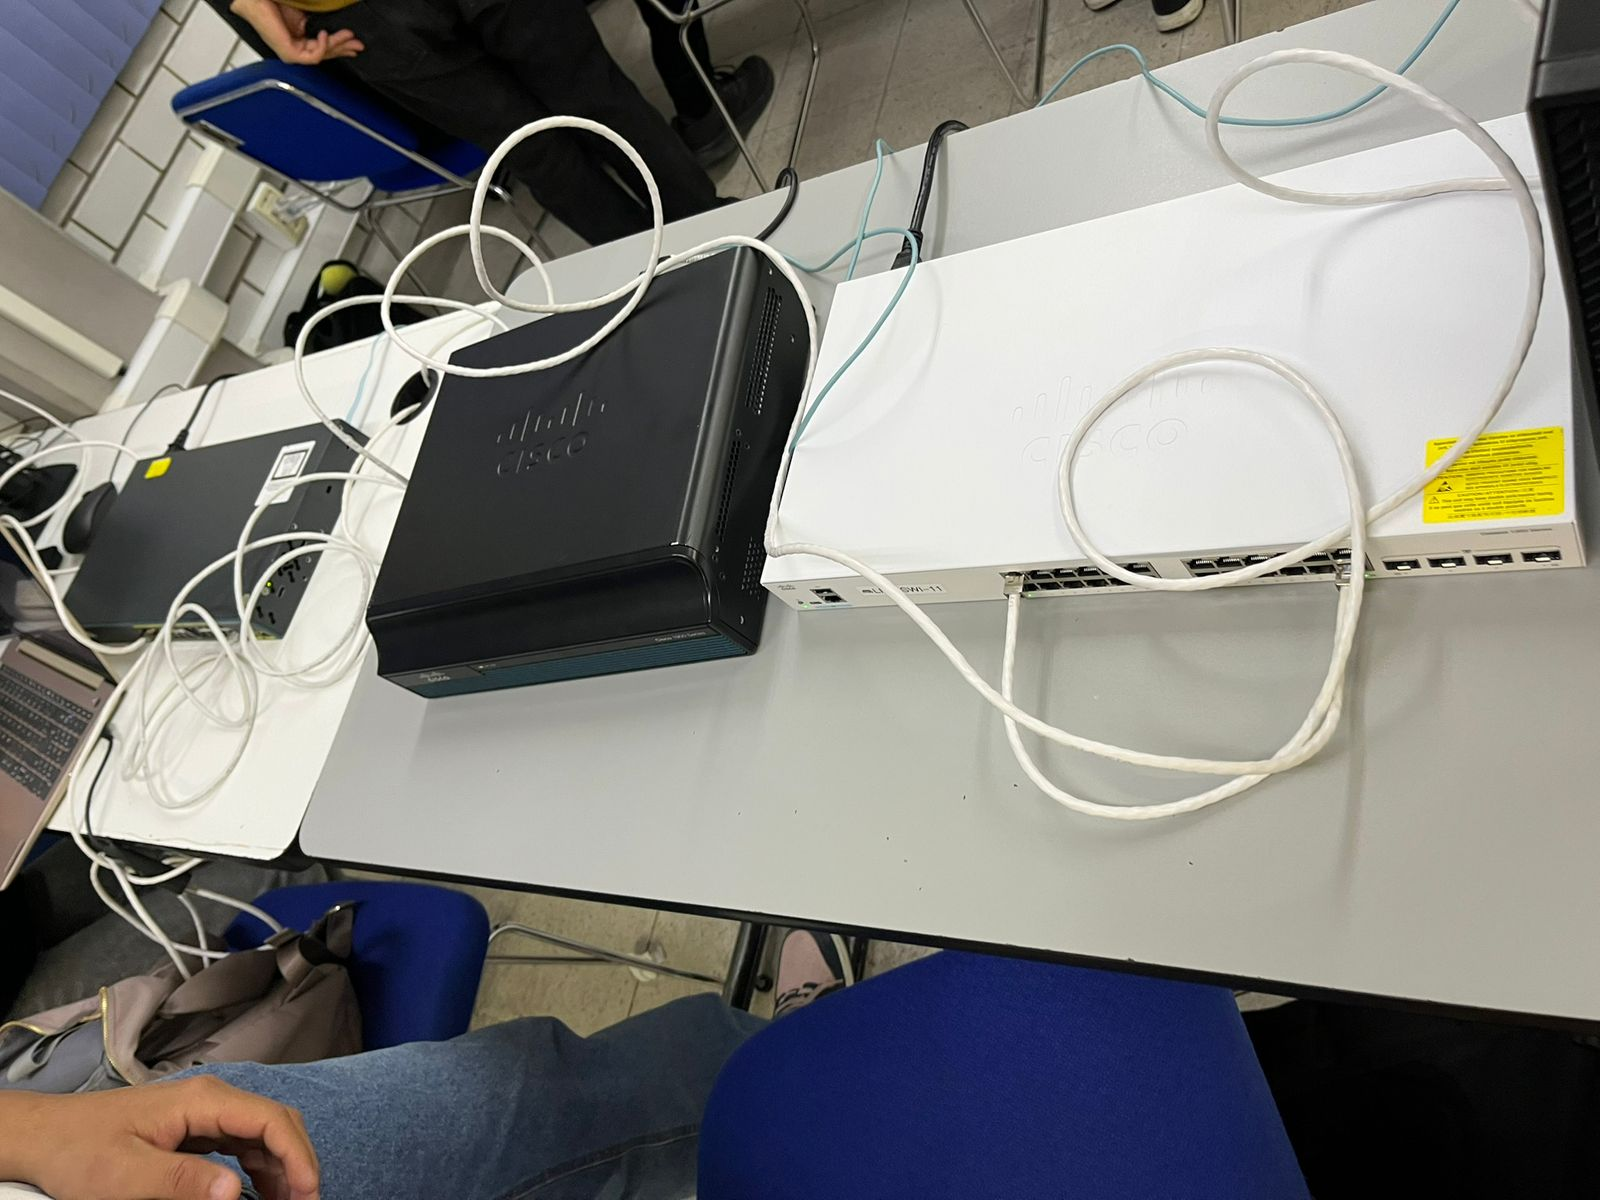
\includegraphics[width=0.8\textwidth]{topologia.jpeg}
  \caption{Topología y cableado de la red en equipo físico}\label{fig:topologia}
\end{figure}

\section{Implementación}

\subsection{Configuración del Router}

Se habilitó el enrutamiento IPv6 con el comando:

\begin{verbatim}
ipv6 unicast-routing
\end{verbatim}

\begin{figure}[H]
  \centering
  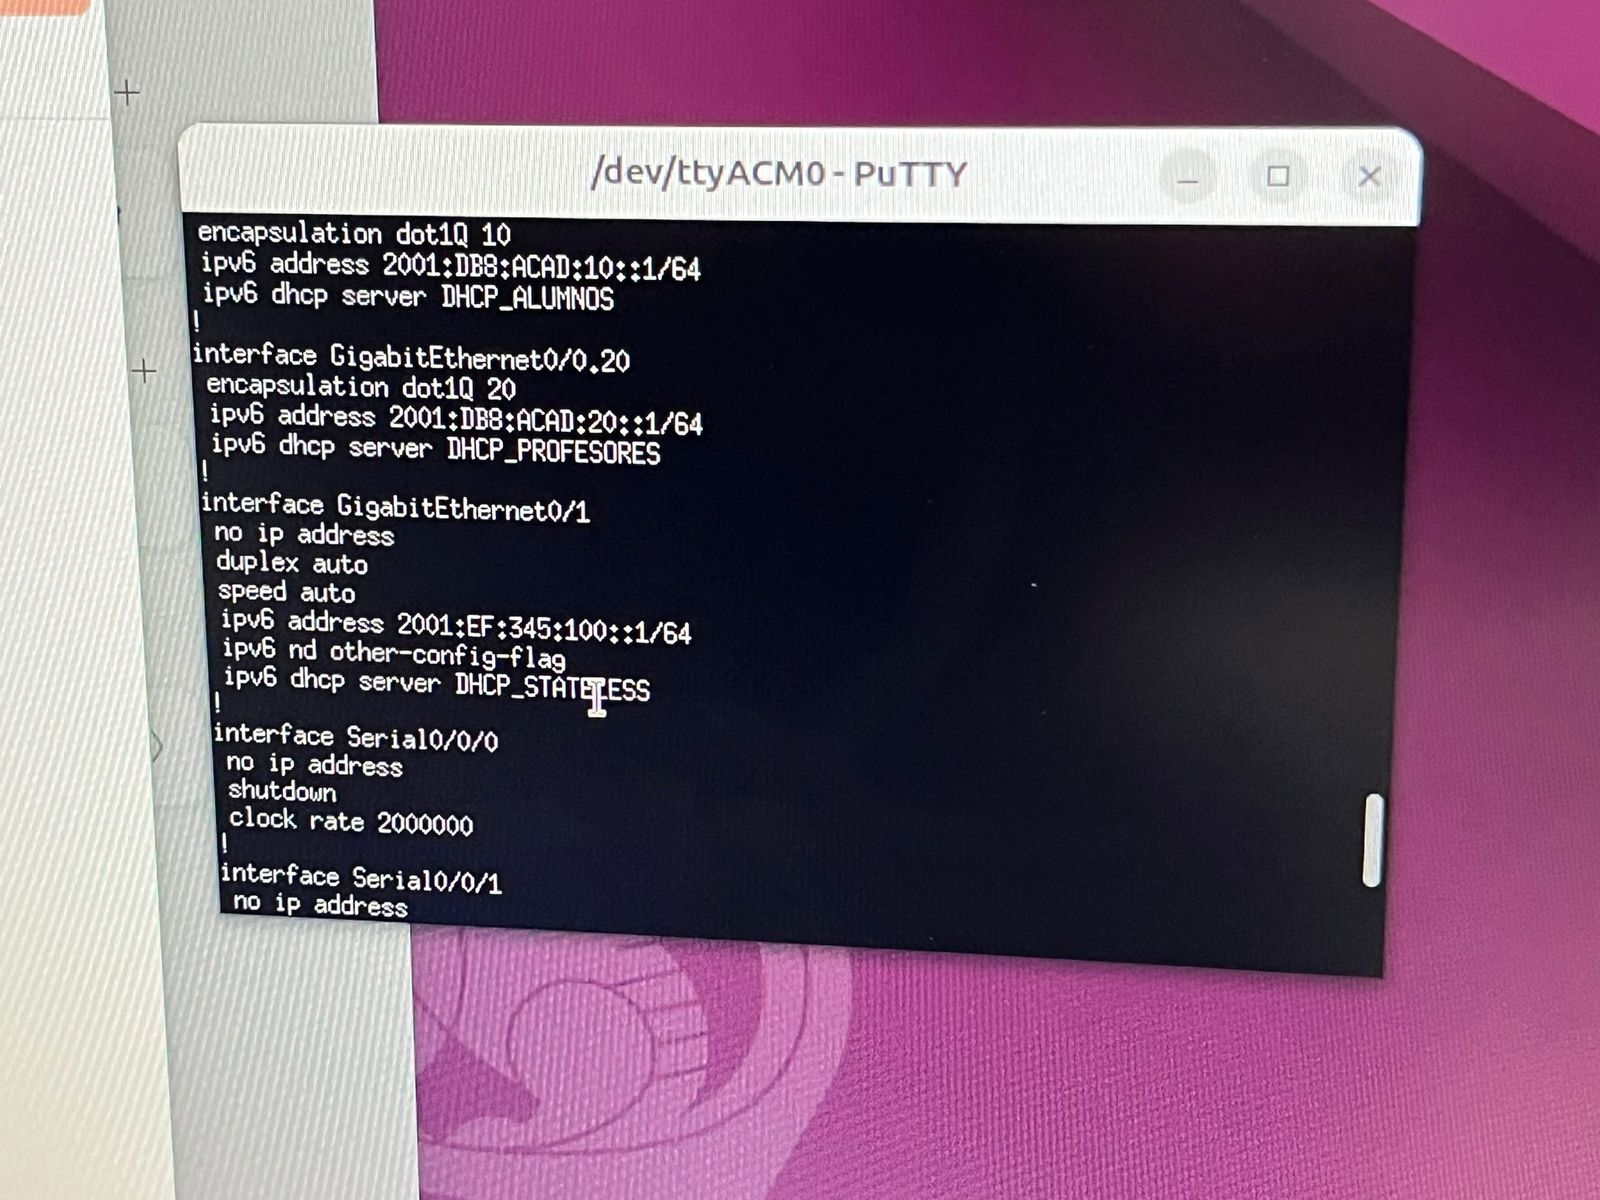
\includegraphics[width=0.8\textwidth]{dhcpv6Config.jpeg}
  \caption{Configuración del DHCPv6}\label{fig:dhcpv6Config}
\end{figure}

\subsubsection{VLAN 10 y VLAN 20 (Stateful)}

Para cada VLAN se configuró una subinterfaz con su respectiva dirección IPv6:

\begin{verbatim}
interface g0/0.10
 encapsulation dot1Q 10
 ipv6 address 2001:db8:acad:10::1/64
 ipv6 nd managed-config-flag
 ipv6 dhcp server DHCP_ALUMNOS
\end{verbatim}

\begin{verbatim}
interface g0/0.20
 encapsulation dot1Q 20
 ipv6 address 2001:db8:acad:20::1/64
 ipv6 nd managed-config-flag
 ipv6 dhcp server DHCP_PROFESORES
\end{verbatim}

Se crearon los pools DHCPv6 correspondientes:

\begin{verbatim}
ipv6 dhcp pool DHCP_ALUMNOS
 address prefix 2001:db8:acad:10::/64

ipv6 dhcp pool DHCP_PROFESORES
 address prefix 2001:db8:acad:20::/64
\end{verbatim}

\begin{figure}[H]
  \centering
  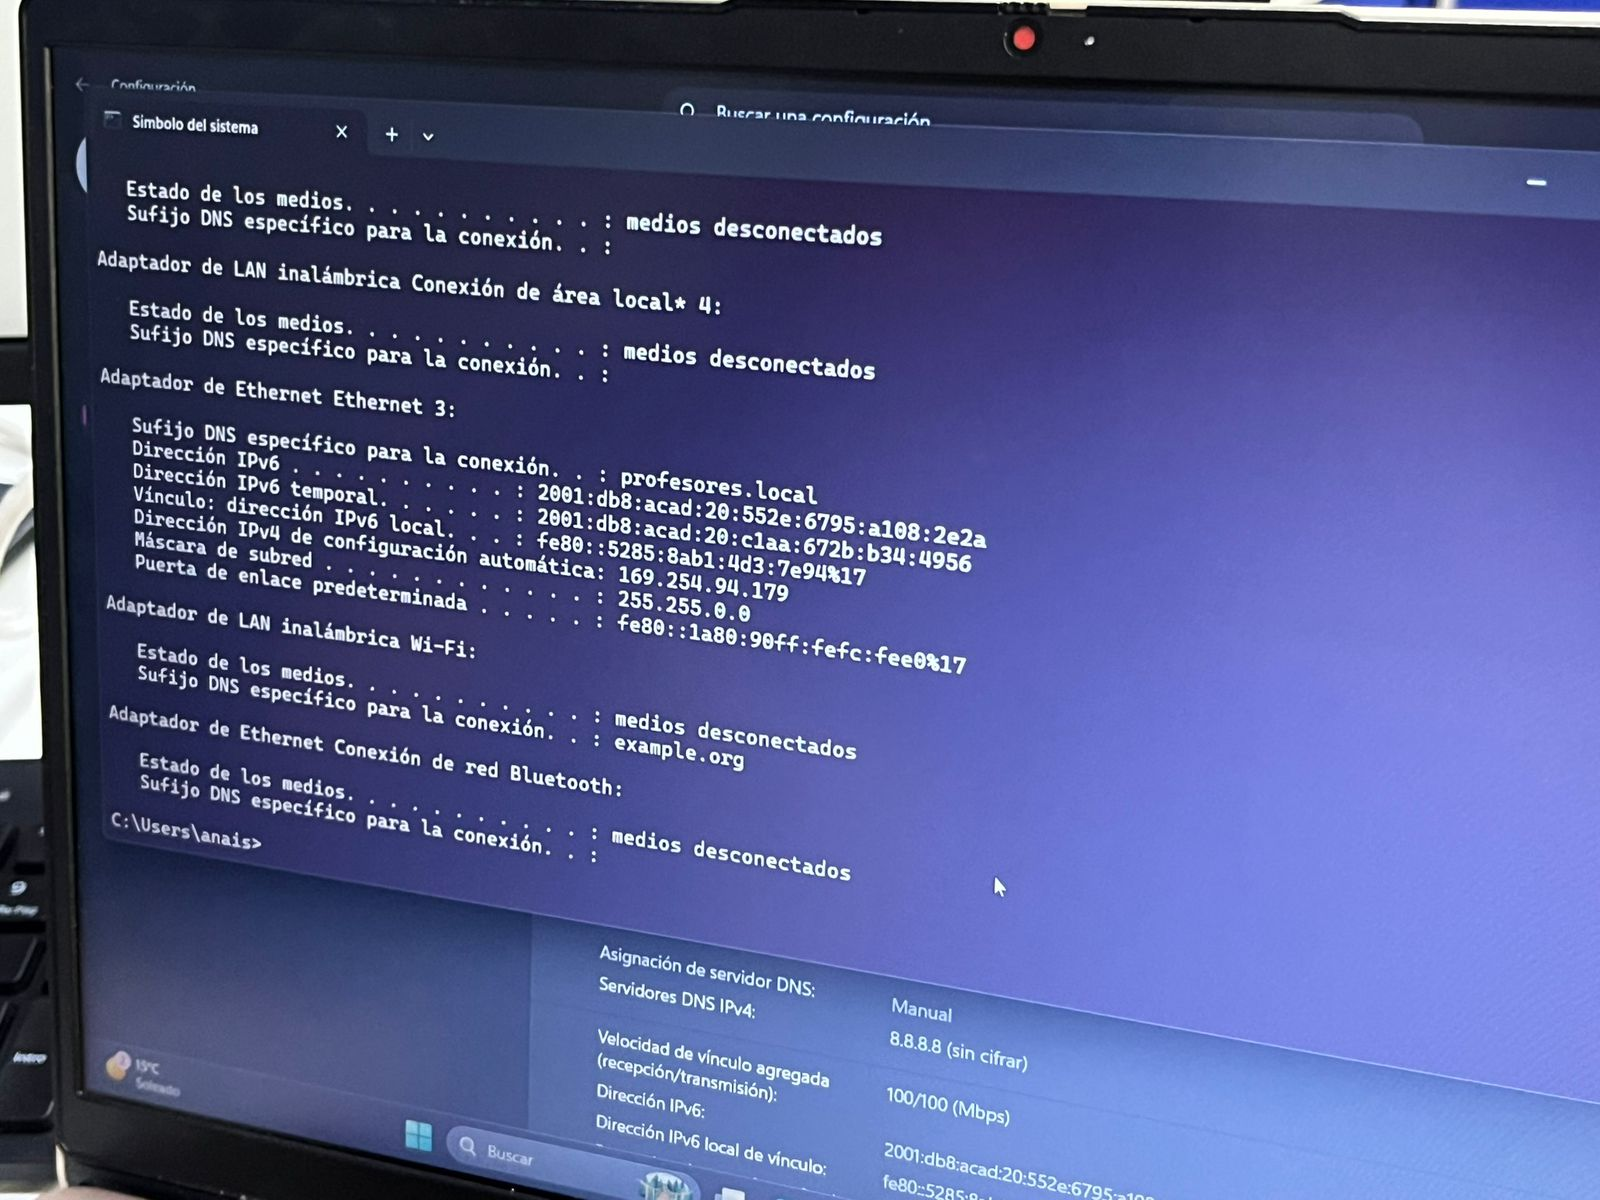
\includegraphics[width=0.8\textwidth]{vlan20.jpeg}
  \caption{Computadora en vlan 20 recibe correctamente su dirección IPv6}\label{fig:vlan20}
\end{figure}


\subsubsection{Lado derecho (Stateless)}

Se configuró una interfaz con DHCPv6 sin estado:

\begin{verbatim}
interface g0/1
 ipv6 address 2001:EF:345:100::1/64
 ipv6 nd other-config-flag
 ipv6 dhcp server DHCP_STATELESS
\end{verbatim}

El pool correspondiente solo proporciona DNS:

\begin{verbatim}
ipv6 dhcp pool DHCP_STATELESS
 dns-server 2001:4860:4860::8888
\end{verbatim}

\begin{figure}[H]
  \centering
  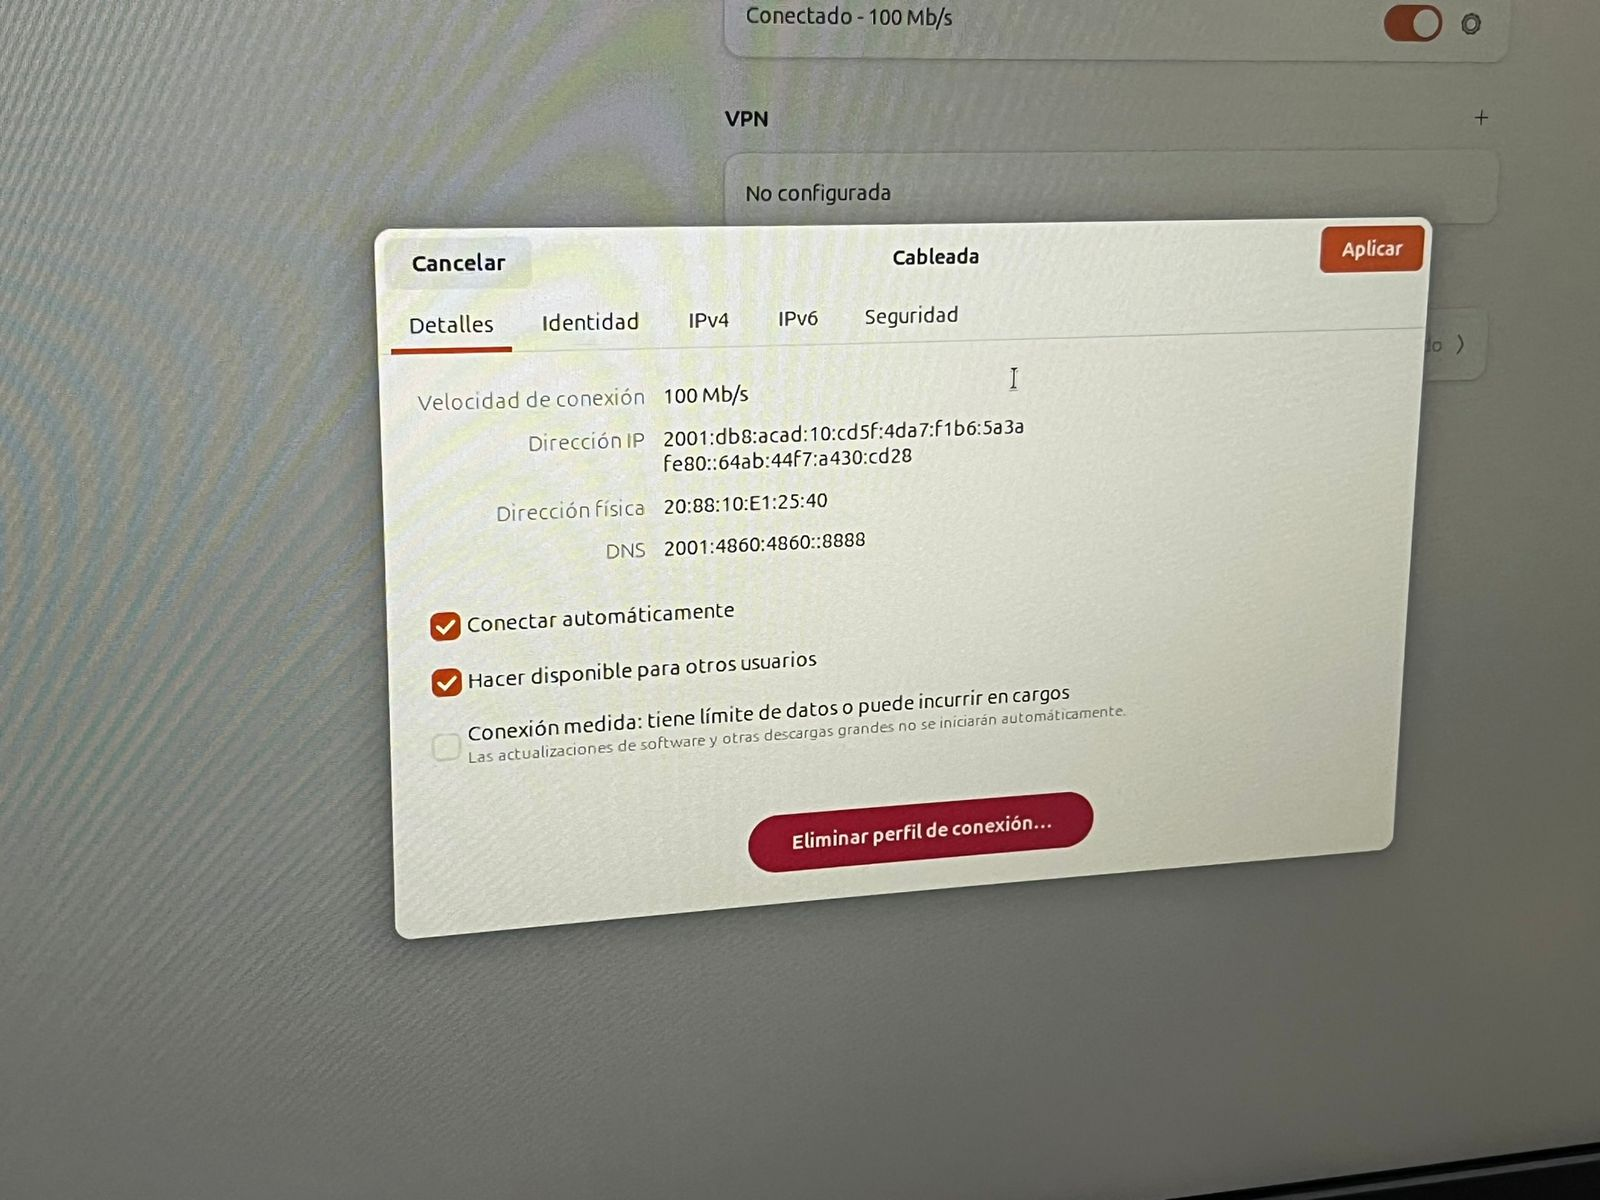
\includegraphics[width=0.8\textwidth]{direccionStateless.jpeg}
  \caption{Computadora en stateless recibe correctamente su dirección IPv6}\label{fig:direccionStateless}
\end{figure}

\begin{figure}[H]
  \centering
  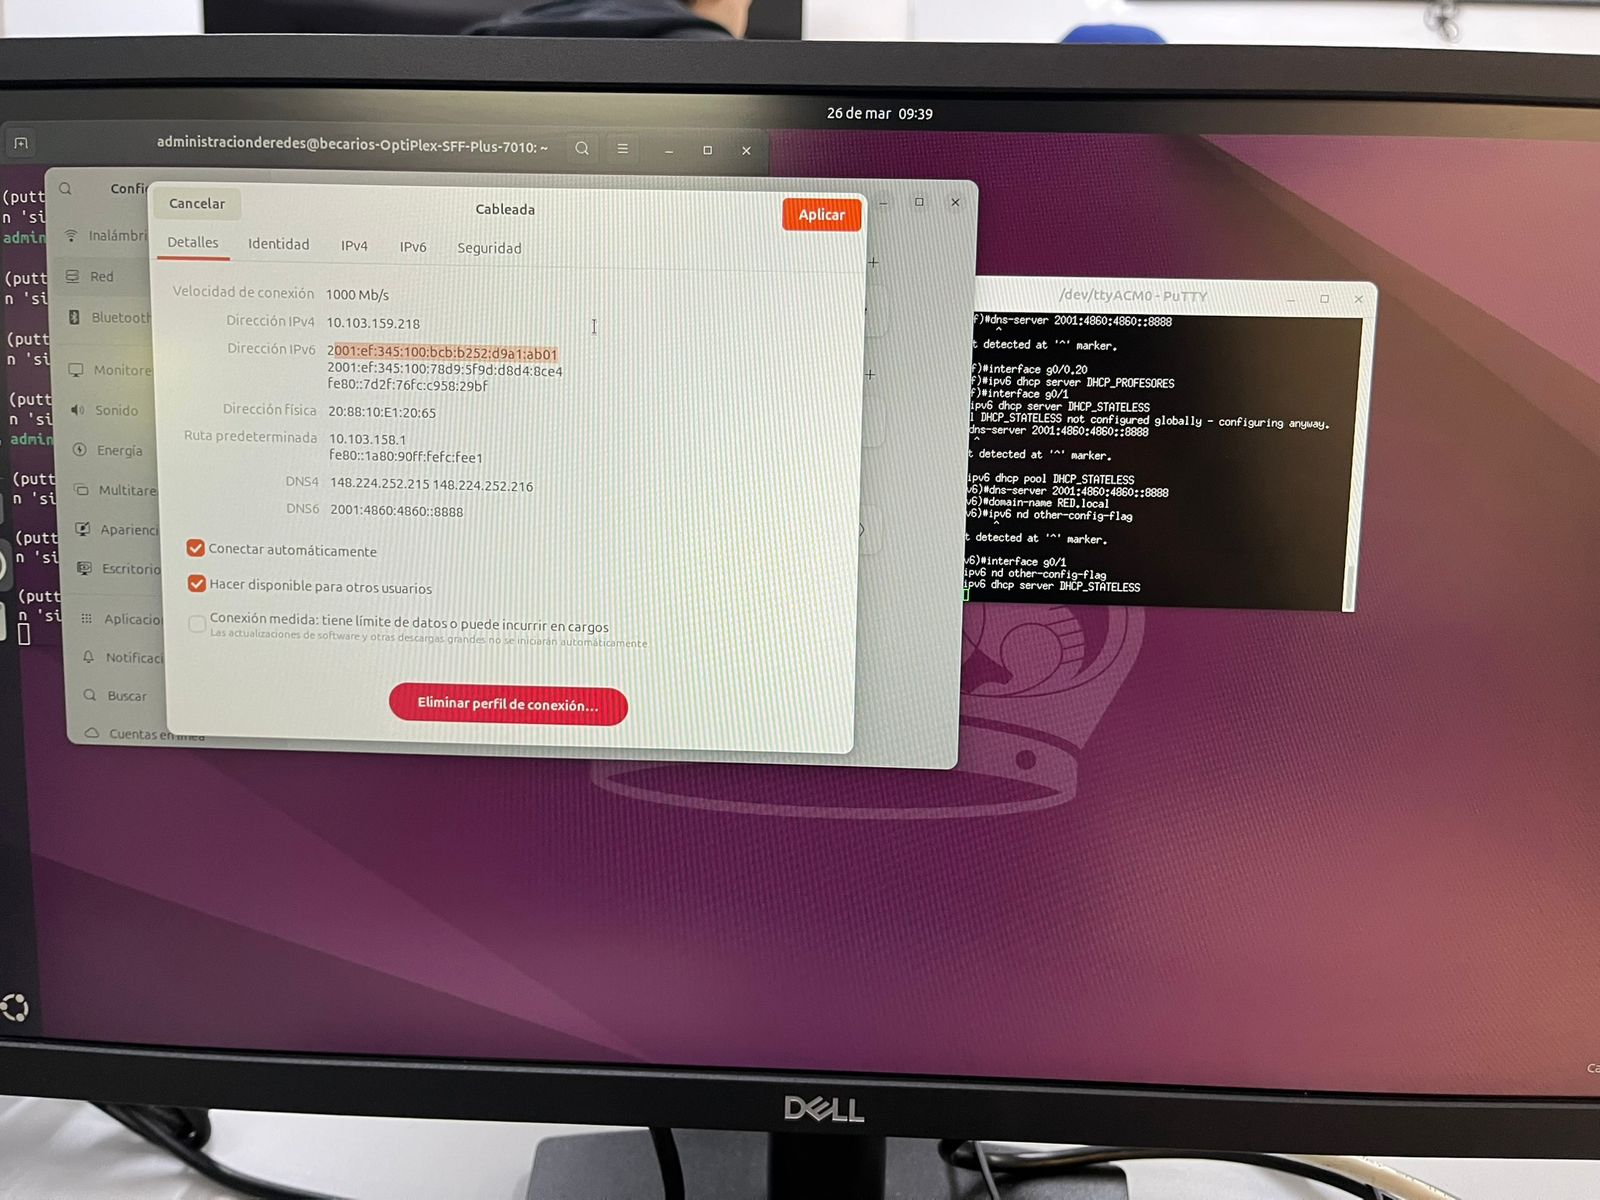
\includegraphics[width=0.8\textwidth]{confyDireccion.jpeg}
  \caption{Consola de configuración de Router y dirección de computadora stateless}\label{fig:confyDireccion}
\end{figure}


\subsection{Configuración de Switches}

En el switch principal se crearon las VLANs y se asignaron los puertos:

\begin{verbatim}
vlan 10
vlan 20
\end{verbatim}

Los puertos hacia las PCs se configuraron como access, y el puerto hacia el router como trunk.

\section{Resultados}

Después de la configuración:

\begin{itemize}
    \item Las PCs en VLAN 10 y 20 obtuvieron direcciones IPv6 mediante DHCPv6 (stateful)
    \item La PC del lado derecho generó su dirección automáticamente (stateless)
\end{itemize}

\section{Conclusión}

La práctica permitió comprender las diferencias entre DHCPv6 stateful y stateless, así como su implementación en una red segmentada con VLANs. 
También se reforzó el uso de Router-on-a-Stick y la importancia de los Router Advertisements en IPv6.

El uso de DHCPv6 facilita la administración de redes al automatizar la configuración de los dispositivos, siendo una herramienta esencial en entornos modernos.

\end{document}
